%% Template written by  Harry H. Cheng
\documentclass[twocolumn,10pt]{asme2ej}

\usepackage{epsfig} %% for loading postscript figures
%structured information, hypotheses, concepts, ideas and approaches

\title{Detecting Spoofed IP Packets using TTL Analysis}

\author{Joseph Faulls
    \affiliation{
	MSci Computer Science\\
    Email: jxf438@student.bham.ac.uk
    }	
}

\begin{document}

\maketitle    

%%%%%%%%%%%%%%%%%%%%%%%%%%%%%%%%%%%%%%%%%%%%%%%%%%%%%%%%%%%%%%%%%%%%%%
\begin{abstract}
{\it At the core of the Internet Protocol lies the datagram, small packets that provide a connectionless communication service across the Internet. These packets contain data such as the sender and receiver's IP address. However, to ensure a quick and connectionless protocol, this information is never validated. This can be exploited and the source IP address forged to any desired to execute a wide array of attacks. This paper discusses a work in progress method to identify IP packets with spoofed source addresses by analysing how long the packet has taken to arrive and comparing this to an expected value. 
}
\end{abstract}

%%%%%%%%%%%%%%%%%%%%%%%%%%%%%%%%%%%%%%%%%%%%%%%%%%%%%%%%%%%%%%%%%%%%%%
\section{Introduction}
The information contained in the header of an IP packet is fundamental to the protocol. Without it, routers would not know where to send it, the receiver wouldn't know where it came from or what protocol it is using, and packets could endlessly circulate the Internet. Therefore, it is required that all datagrams contain a source and destination address, the protocol used, a checksum to validate the integrity of the header, and a lifetime \cite{rfc791}.

Although, because datagrams are connectionless, there is no way to validate the correctness of the source address just by looking at the header. Faking the source of a packet is known as IP Spoofing, and is already a well established problem \cite{ipSpoofIntro} \cite{ipSpoofing} \cite{spoofProblemStatement}. This can be achieved very easily through the use of off-the-shelf programs such as {\it hping}\cite{hping}, where faked packets can be forged in a single line command.

The motives to spoof an IP packet are almost exclusively malicious. The primary reason would be to conceal the origin of an attack - seeing as most systems keep logs of their Internet activity and IP addresses can be traced back to their physical location. However, this goes much further than just simply masking identity; many serious attacks rely on IP Spoofing. These are discussed in detail in section \ref{attacks}.

Efforts have already been made to combat IP Spoofing to some degree of success. However, many of the techniques are difficult/costly to implement or have been made no longer possible. These are outlined in section \ref{defences}. This paper discusses the progress and theory behind an alternate, low-cost, passive approach to identify spoofed packets through the use of machine learning techniques. 

Earlier, it was mentioned that IP headers must include a lifetime, or Time To Live (TTL), to prevent data circulating a network or computer indefinitely. This is represented as an 8-bit decrementing counter of how many times the packet has hopped between routers. Upon reaching 0, the data is discarded.

Based on the assumptions that the route taken by separate requests from the same source are the same, or very similar, we can expect similar TTL values from a given source through all requests. Therefore, if a packet arrives with a TTL value statistically different enough from the expected one for the given source address, we can assume that the packet has taken a very different route to get there. Consequently, the source address was probably spoofed.

The problem now lies in how do we calculate an expected Time To Live? A naive approach would be to send a small request to the apparent source address and compare the TTL of the response to that of the request. This technique is clearly a very costly one and would increase the time taken to receive and accept the packet by a factor of roughly three. 

More intuitively, we can log all the source addresses and TTL values for all incoming packets. Over time, a large database or map can be generated with expected values for all seen IP addresses. Then, when a request comes in, it's TTL is compared to ones seen before from that address.

The main limitation to this method is clear, what is to be done with an unseen address? A simple one-to-on mapping of IP addresses to expected packet is too specific, it cannot be assumed that malicious traffic would contain a spoofed source address that has been previously seen by the server. Therefore, a mechanism to predict an expected TTL value for unseen source addresses is required. Perhaps clustering IP addresses to similar physical location.

Currently, very limited resources have been spent researching a system to cluster and classify the correctness of source IP addresses. Therefore, this paper will focus on the surrounding literature, along with the method and implementation of a program to collect and store incoming traffic data efficiently at high load.

%%%%%%%%%%%%%%%%%%%%%%%%%%%%%%%%%%%%%%%%%%%%%%%%%%%%%%%%%%%%%%%%%%%%%%
\section{Attacks Using IP Spoofing} \label{attacks}

Being able to fake the source of IP packets not only conceals the attacker, alleviating risk of being caught, but also plays a fundamental role in enabling a wide array cyber-attacks. Several of these methods will be explored into some depth to demonstrate how they could all be avoided if spoofed IP addresses could be identified and discarded.

One attack not strictly related to IP spoofing, but worth mentioning, is an IP or network routing attack. This is where a router makes false claims about itself to have traffic diverted towards it, usually for some malicious purpose. Perhaps it claims to have direct links with far away routers, making it a preferred choice. This ultimately changes the route (thus, the average TTL) and allows passive spoofed packet detection using TTL to also act as a routing change detector. 

%%%%%%%%%%%%%%%%%%%%%%%%%%%%%%%%%%%%%%%%%%%%%%%%%%%%%%%%%%%%%%%%%%%%%%
\subsection{SYN Flood}
First discovered in 1996, the TCP SYN flood is a notorious and common method of a denial-of-service (DoS) attack \cite{rfc4987}. The prime objective, as with all DoS attacks, is to exhaust the host's network resources such that it is unable to service legitimate requests. This is accomplished by taking advantage of the three-way handshake, the TCP connection establishment process.

\begin{figure}[h]
	\begin{center}
		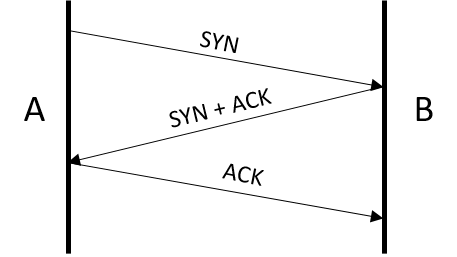
\includegraphics[width=4.57cm, height=2.57cm]{figures/three-way-handshake}
	\end{center}
	\caption{TCP three-way-handshake}
	\label{figure_handshake} 
\end{figure}

After receiving the first SYN request, the host B sends the SYN+ACK packet and enters into a listening state, waiting for the final ACK. If the initial SYN request had a spoofed source address, this packet would be sent to a different machine than the one that started the handshake. Therefore, the host B will never receive the final acknowledgment packet and just keep waiting until a timeout. 

Although the data structure to hold the current state is relatively small, this soon adds up as more half-open connections are created, eventually causing the server to be unable to accept any more requests - denying legitimate users.

%%%%%%%%%%%%%%%%%%%%%%%%%%%%%%%%%%%%%%%%%%%%%%%%%%%%%%%%%%%%%%%%%%%%%%
\subsection{TCP Session Hijack}
Interrupting and exploiting a valid computer session to pose as the trusted client is known as session hijacking. The TCP protocol makes this difficult to do by generating an initial sequence number (ISN). For a connection to be established, the two TCPs must synchronise on each others ISN, and the reply packets must include the ISN of the preceeding packet \cite{rfc793}. 

Therefore, for an attacker to hijack the session, they must first acquire the sequence number and ensure they get the replies back before the target. The latter of this can be done through a denial-of-service attack. 

The job of acquiring the ISN is more challenging. If the attacker were on the same segment as the victim, this is a trivial job accomplished by sniffing packets. However, without access to the network traffic, the attacker must predict the sequence number. This can be done by exploiting the generation process or performing an rsh server attack \cite{tcphijacking}.

Even if the attacker goes through the trouble of acquiring the ISN one way or another, the requests to the server must be spoofed to pose as the victim and the average TTL will suddenly change. If this sudden change in TTL can be identified, the connection can be shut down and this attack can be nullified completely.

This is a unique attack in the fact it uses IP spoofing with TCP rather than the more attractive connectionless UDP packets. Techniques have already been developed to combat this with high degree of success. Network level hijacks can be prevented by encrypting the packets using any of the widely available protocols such as SSL or SSH.

%%%%%%%%%%%%%%%%%%%%%%%%%%%%%%%%%%%%%%%%%%%%%%%%%%%%%%%%%%%%%%%%%%%%%%
\subsection{Reflective UDP Amplification}
Denial-of-service attacks often employ reflective UDP amplification to disrupt networks and systems. This technique allows for a server to amplify the malicious traffic whilst concealing the source of the attack.

Targeted servers used to reflect the traffic can either be rented or any other an attacker can find running applications that use connectionless protocols (like DNS or SNMP) and do not require authentication from their clients. Using multiple servers is desirable so that the malicious packets arrive from distributed sources. This means the victim cannot block all attack packets by blocking one server. This is known as a distributed denial-of-service attack.

To get traffic to arrive at the victim, UDP request packets are sent to a server with the source address spoofed to be that of the victims. Therefore, the victim receives the reply packets, perhaps many times bigger than the small request packet sent. This means that the attacker can generate attack flows of many tens of Gb/s whilst only sending 1 Gb/s of traffic themselves.

\begin{figure}[h]
	\begin{center}
		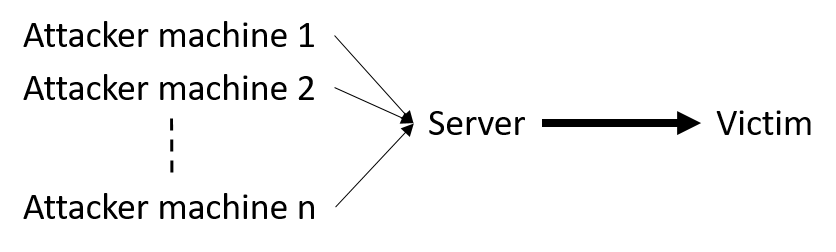
\includegraphics[width=8.36cm, height=2.52cm]{figures/udp-amplification}
	\end{center}
	\caption{Reflective UDP Amplification}
	\label{figure_amplification} 
\end{figure}

Due to the effective and highly accessibly nature of the attack, US-CERT (United States Computer Emergency Readiness Team) issued an alert on UDP-based amplification attacks in 2014 \cite{USCERT}.
%%%%%%%%%%%%%%%%%%%%%%%%%%%%%%%%%%%%%%%%%%%%%%%%%%%%%%%%%%%%%%%%%%%%%%
\subsection{Smurf Attack}

This is distributed denial-of-service attack (or DDoS - meaning the abusive traffic arrives from many different computers at the same time), in which the spoofed IP address is that of the victim's. Large numbers of Internet Control Message Protocol (ICMP) packets with the victim's source address are broadcast to computer network using an IP broadcast address\cite{rfc919}. Every machine on the network will attempt to send a reply to the source address, thus flooding the victim with traffic \cite{smurf}. 

\begin{figure}[h]
	\begin{center}
		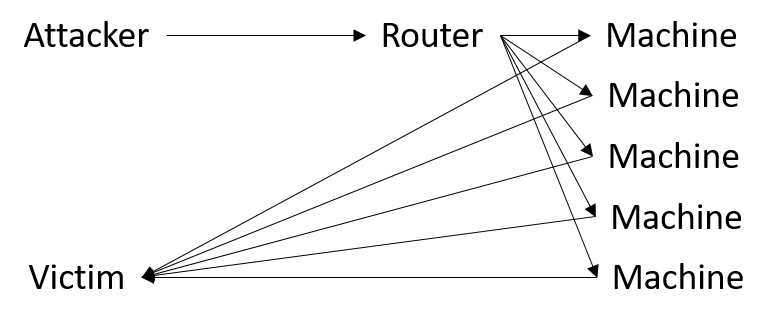
\includegraphics[width=7.67cm, height=3.22cm]{figures/smurf}
	\end{center}
	\caption{Smurf Attack: how one request can lead to hundreds}
	\label{figure_smurf} 
\end{figure}

%%%%%%%%%%%%%%%%%%%%%%%%%%%%%%%%%%%%%%%%%%%%%%%%%%%%%%%%%%%%%%%%%%%%%%
\section{Related Work} \label{defences}

Efforts to prevent spoofed IP packets from being processed and regarded as legitimate can be categorised into active and passive methods. Both methods can either be implemented on a router or host level. 

Active methods attempt to verify the legitimacy of the source address by either tracing the packet, or detecting whether the supposed source was able to originate where it physically arrived from. However, passive methods simply classify a packet as being legitimate or not, and do not verify the actual source so cannot be used to establish accountability for attacks. The majority of work done to identify spoofed packets are active methods.

%%%%%%%%%%%%%%%%%%%%%%%%%%%%%%%%%%%%%%%%%%%%%%%%%%%%%%%%%%%%%%%%%%%%%%
\subsection{Eliminating Spoofed Packets from the Internet \cite{eliminating}}
Published in 2007 by the IETF Trust, this approach was motivated by the Source Address Verification Architecture Problem\cite{spoofProblemStatement}, a formalisation of the IP spoofing problem. Implemented at a router level, this method attempts to detect and discard any datagrams with spoofed addresses by devices that have an authoritative mapping between IP addresses and the network topology. Discarding spoofed packets at the earliest stage possible prevents any from circulating the Internet, nullifying any need to analyse packets at a host level.

A device that is close enough to the source to have a table between layer 2 (Data link layer) and IP addresses can discard any packets in which the IP address is not associated with (and is therefore assumed to be spoofed) the layer 2 address in the datagram. This device can be a CPE router (Customer Premise Equipment), ISP PE router (Premise Edge, meaning a router between one network service provider's area to outside their premise), NNI router (Network-to-network router providing interconnections of provider's networks), switch or a host.

\begin{figure}[h]
	\begin{center}
		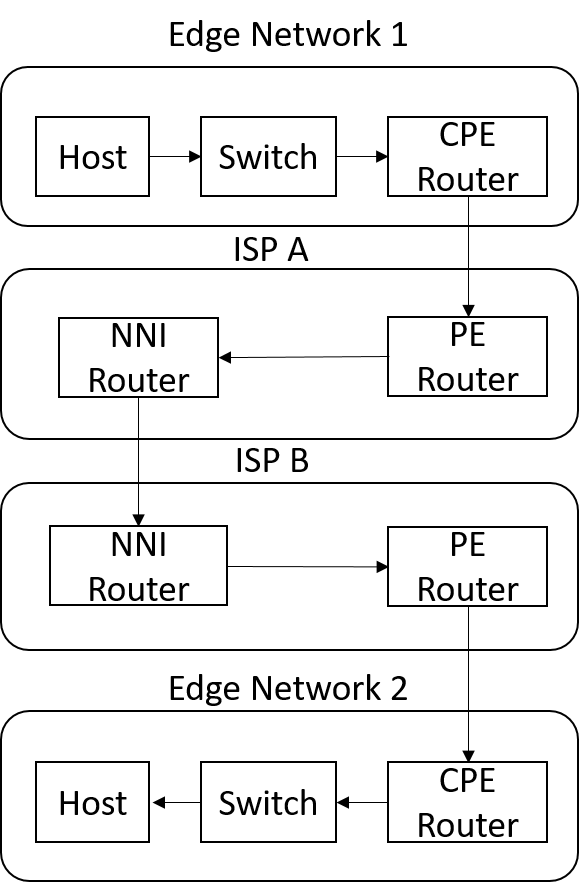
\includegraphics[width=5.79cm, height=8.82cm]{figures/eliminating2}
	\end{center}
	\caption{This illustrates five locations a source address can be validated: Host to Switch, Switch to CPE, CPE to ISP PE, ISP NNI to ISP NNI and ISP PE to destination CPE}
	\label{figure_eliminating} 
\end{figure}

For ISP Premise Edge routers, RFC 2827 \cite{rfc2827} encourages ISP's to use ingress filtering. This is as simple as the router checking if the source IP of a packet coming from a machine residing in, for example, \texttt{204.32.123.0/24} actually falls in this range. If it does not, the packet is discarded and the suspicious behavior is logged.

An advantage of this is that the origin of malicious datagrams can be determined and responsibility assigned. However, implementing such a technique is a widespread, collaborative solution to solving IP spoofing. This must be used everywhere for it to be effective. For example, the ISP might include an agreement in its service contract to use this procedure in its supplied router.

%%%%%%%%%%%%%%%%%%%%%%%%%%%%%%%%%%%%%%%%%%%%%%%%%%%%%%%%%%%%%%%%%%%%%%
\subsection{IP Source Guard \cite{ipsourceguard}}

Another router level implementation, this feature attempted to become a best current practice for defeating denial-of-service attacks in a switched LAN environment. It provides protection by limiting specific port access to clients that have received an IP address from the DHCP server (a standard network protocol to dynamically distribute IP addresses), rendering packet spoofing within the network impossible. 

However, the problem with implementing this on a router interface, is that illegitimate data will simply be discarded without advising the network or the user. Additionally, it is perfectly legal for a host to have more than one IP address. It is entirely possible that datagrams are sent using an IP address different from the interface's primary one. This would get discarded by the router and no error message returned.

This solution, although very effective, would only work for IP packets being spoofed as ones coming from inside the local network. This eliminates any local IP address authentication systems, but does not stop spoofed packets coming from outside the network.


%%%%%%%%%%%%%%%%%%%%%%%%%%%%%%%%%%%%%%%%%%%%%%%%%%%%%%%%%%%%%%%%%%%%%%
\subsection{Detecting Spoofed Packets \cite{dsp}}

Motivated by the messy variety and lack of an industry standard solution to the IP spoofing problem, S. J. Templeton and K. E. Levitt published a paper in 2003 discussing the attacks and various methods of detecting spoofed packets. They provided both active and passive approaches, as well as presenting results of experiments to verify the effectiveness of passive methods. 

Most notably, passive TTL methods were explored, based on the same assumptions in this paper. The intuition for the approach was much the same, that packets coming from the same source should have similar TTL values, and if an anomalous packet is observed, then it may well be spoofed. However, no method for predicting expected TTL values for previously unseen IP addresses was implemented.

IP data was collected over a 2 week period, with over 23,000 unique IP addresses recorded. Using Conditional Entropy as an indicator of how predictable a TTL value was for a given source address, their conclusions indicated that TTL values appear to be highly predictable and thus can be the basis for spoofed packet detection. Although The accuracy was never tested, it was proposed that it is a good indication and can be used in conjunction with other methods as a first line of defence.

The paper concluded that 'no current detection method is 100\% correct'. Yet this does not devalue their utility, improvement is better than nothing. With a combination of more than one defence can greatly increase the effectiveness of identifying spoofed packets.

%%%%%%%%%%%%%%%%%%%%%%%%%%%%%%%%%%%%%%%%%%%%%%%%%%%%%%%%%%%%%%%%%%%%%%
\subsection{Encoding Route Information Into Packets \cite{traceback}}
For practical deployment of IP traceback techniques, it was suggested that the IP identification field of IPV4 headers (primarily used for uniquely identifying groups of fragments of a single IP datagram, a practice that is not often used) could be overloaded to encode edge fragments. This meant that victims of IP spoofing could identify the network path traversed by the packets without requiring interactive suppose from the ISP.

Although promising work, RFC 6864 has since updated the IPV4 specification in 2013 to strictly forbid using the Identification field for any other purpose than what it was intended for \cite{rfc6864}.

%%%%%%%%%%%%%%%%%%%%%%%%%%%%%%%%%%%%%%%%%%%%%%%%%%%%%%%%%%%%%%%%%%%%%%
\section{Limitations of a TTL Based Method}
Although a low-cost, passive approach to the IP-spoofing problem, solely relying on the TTL field in packet headers is not a definitive technique for identifying spoofed source addresses. Exactly how effective this method is, is not currently known and will hopefully be quantified soon. Yet there are situations where TTL analysis cannot be used.

\subsection{Similar Location or Routes}
If the source address is faked to be one close by, perhaps the same sub network, then the TTL will be roughly the same and may not be statistically different enough to be classed as taking a different route to arrive. This is also the case if the faked source would take a similar amount of hops to the server than the attacker's packet would. Unfortunately, this would be impossible to detect looking at TTL alone.

However, being on the same sub network might raise suspicion as large streams of data would either be, depending on the attack, contained within the network or entering and exiting the network simultaneously.

\subsection{Differing Initial TTL Values}
Furthermore, different protocols use different initial TTL values. So simply comparing TTL's is not a viable option. Thankfully, the set of default TTL values for protocols is small. In almost all cases, default values are very commonly either 64 and 128 for TCP/UDP, or 128 and 255 for ICMP (Internet Control Message Protocol). Knowing this, we could make accurate educated guesses as to what the initial TTL value was set to. For example, if we observe the following closely grouped data from a given source address: \texttt{4x57, 8x58, 10x121, 23x122}, we can assume the values in the high 50's had an initial TTL of 64, whilst low 120's started at 128. This means that packets took 6-7 hops in all cases.

\subsection{Faking TTL Values}
Of course, like the source address, TTL fields can be set to whatever the sender chooses it to be. However, to fake a TTL to mimic that of what the spoofed source's would look like, the attacker must know or make very advanced approximations to the route taken from the fake source to the victim. This is a very hard, if not impossible, task to accomplish. And seeing as many attacks using IP spoofing use a wide array of spoofed addresses throughout their packets, this must be calculated for every spoofed address.

\subsection{TTL Prediction for Unseen IPs}
It is not reasonable to assume the database will always contain a given source addresses. Therefore, generating an expected TTL value for a source address cannot solely rely on previous data from the same source. A mechanism to predict TTL values for unseen addresses is desirable. For starters, the tool can only look at the first 24 bits of the address, allocated for the network prefix. The last 8 bits are reserved for host addressing, so we can assume that all IP addresses that only vary by these 8 bits are physically very close together, so TTL values will be very much the same.

In conjunction with this, the basic method for attaining an accurate TTL referred to in section 1 could be an effective way to deal with previously unseen IP addresses. This is to simply send a request to the supposed source IP and compare the TTL values of the response and packet in question. Although this will take longer, it only must be used once on unseen addresses. Subsequent requests from the same source will not be hindered by this check.

However, denial-of-service attacks that IP spoofing typically choose fake source addresses at random from the entire IP address space. A side affect of this is that many of generated addresses them will be unreachable. IP packets with such addresses are known as 'bogons'. These typically include ones that are not in the range of allocated addresses by the Internet Assigned Numbers Authority (IANA), ones not delagated by regional Internet Registry that are allowed for public Internet use, or addresses privately reserved\cite{rfc1918}. Trying to calculate an expected TTL for such addresses is impossible, as the request will never reach a machine.

Standard DDoS protection tools can detect if an IP address is unreachable and can categorise it as spoofed. This means bogon filtering can be used in conjunction with this method to prevent trying to calculate TTL's for unreachable addresses. However, to work around bogon filtering, more sophisticated spoofing tools avoid unreachable addresses. Thankfully, this increases the chance that the spoofed source has been observed before.

%%%%%%%%%%%%%%%%%%%%%%%%%%%%%%%%%%%%%%%%%%%%%%%%%%%%%%%%%%%%%%%%%%%%%%
\section{Data Collection}

To determine the predictability and to generate expected TTL values, large quantities of traffic data must be gathered and analysed. A significant challenge of the project is to build and implement a tool to do exactly this. Straightforward approaches to log traffic are available, for example iptables \cite{iptables}, a command line utility for configuring a Linux kernel firewall implementation. However, this is a large tool and struggles processing high volumes of data efficiently.

It was agreed that the School of Computer Science would be willing and able to help with data collection. A port mirroring all traffic to one of their machines could be supplied. As the tool only logs source IP addresses, protocol and TTL values - all packet data is discarded, preserving the data's integrity, meaning no ethical issues were raised. Originally, a mirror virtual machine was to be supplied - however, initial testing revealed all IP packets have their TTL values set to 64 when traversing the gateway network between the host and virtual machine.

The University of Birmingham School of Computer Science connections vary from 1gb/s to up to 10gb/s transfer speed. Ideally, the fastest speed would be desirable, providing more data. However, if the logging program is unable to handle such high speeds, it can simply be run on a machine with a slower transfer rate. This, once again, highlights the critical need for efficient data structures and operations.

%%%%%%%%%%%%%%%%%%%%%%%%%%%%%%%%%%%%%%%%%%%%%%%%%%%%%%%%%%%%%%%%%%%%%%
\subsection{Netfilter\cite{netfilter}}
Linux distributions provide a very useful packet filtering framework called Netfilter, allowing for fully customisable networking operations through the use of hooks. This enables kernel modules to register callback functions with the network stack. The function is then called for every packet that traverses the hook. One of the more popular features of Netfilter is the aforementioned iptables.

All of the Netfilter operations are done in kernel space, eliminating the need for costly translation of data between kernel and user space. However, developing and running in kernel space also has its disadvantages. For example: software bugs, such as memory errors, lead to kernel panics, requiring hard resets of the machine; some standard c functions are unavailable; and error messages and stack traces are difficult to interpret.

%%%%%%%%%%%%%%%%%%%%%%%%%%%%%%%%%%%%%%%%%%%%%%%%%%%%%%%%%%%%%%%%%%%%%%
\subsection{Utilising Threads}
To be capable of handling intense data loads, the time taken from receiving to accepting an IP packet must be minimised. If all operations to record the data were done on a single thread, then the process must wait for the data to be stored before it can let the packet through and start looking at the next one. Under high loads, this could result in packets being lost due to overflowing the available memory, violating the legitimacy of the data collected. Intuitively, concurrent execution must be utilised.

An initial strategy would be to simply start a kernel thread (kthread) in the netfilter hook callback function, passing the necessary data to be stored. However, the callback functions operate in interrupt context, and creating a kthread implicitly creates a thread scheduler that may sleep. Seeing as sleeping is strictly forbidden in interrupt context, this method will not work.

A neat solution to this problem are workqueues, a generic asynchronous execution mechanism \cite{workqueue}. Superficially, they allow kernel code to request that function be called at some time in the future. More importantly, adding work to a queue can be done in interrupt context so that it can be dealt with later, by another thread.

\begin{figure}[h]
	\begin{center}
		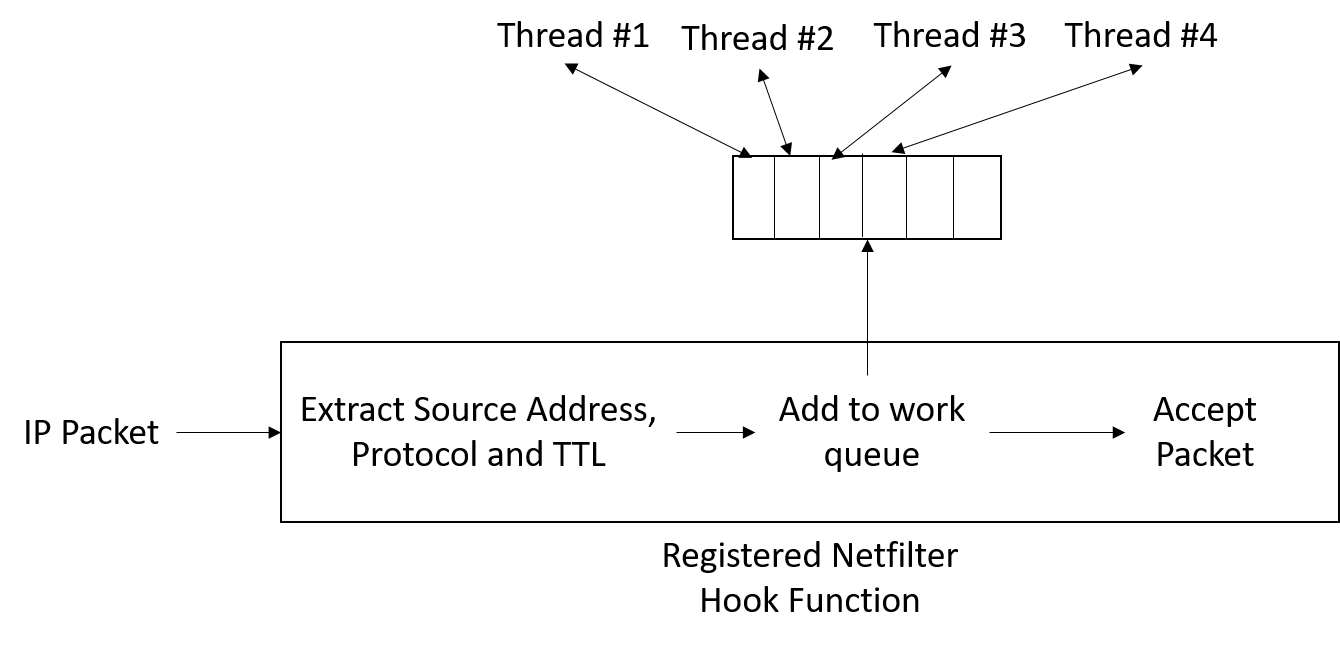
\includegraphics[width=7.37cm, height=3.55cm]{figures/workqueue}
	\end{center}
	\caption{Multiple threads take work out of the workqueue concurrently without delaying the packet flow}
	\label{figure_workqueue} 
\end{figure}

Most notably, it is possible to initialise a workqueue to have one dedicated kthread for each processor on the system. This further utilises all available computing power: not only can we separate the hooking from the processing of the data, but we can also separate the processing by having multiple threads taking work out of the workqueue and handling the data concurrently.

%%%%%%%%%%%%%%%%%%%%%%%%%%%%%%%%%%%%%%%%%%%%%%%%%%%%%%%%%%%%%%%%%%%%%%
\subsection{Storing the Data}
It was mentioned that the Netfilter hook function operates in Kernel space, and that moving data from Kernel to userspace is costly. It follows that, to have the program run as fast as possible, the logging of the data should be executed in kernel space, and infrequently transfer over to into userspace in large chunks to be stored permanently This can be done perhaps once every 5 minutes, or when the kernel is close to running out of memory. The disadvantage to this technique is that in the case of the machine failing (e.g. power cut), a maximum of 5 minutes of data will be lost.

\subsubsection{Kernel Space}
To store a relatively small amount of data (5 minutes worth) in Kernel space, not only is an efficient data structure most desirable (discussed in depth in section \ref{data_structures}), but the amount of data stored for each logged packet should be as quick as possible to construct and handle. Regardless of structure, each node of data should contain the source address, protocol and observed TTL values. 

Source addresses are supplied as an unsigned 32-bit integer and have to be transferred into the usual human readable character array format, such as \texttt{192.168.0.1}. However, transferring it into this format is counter-productive, as it not only costs to do, but operations to compare addresses in character arrays is far less efficient than comparing integers. Similarly with the protocol, this is unsigned 8-bit integer and can remain so to improve efficiency.

Storing observed TTL values is more complicated, as there will be many values for one address. The most basic data type to deal with multiple values is having a fixed block of contiguous memory locations known as an array. However, storing one value for each packet is difficult to manage as it is not known how much memory to reserve when creating the array. A far better solution is to have an array of integers of size maximum TTL value (255, being an 8-bit integer), and each element of the array being the number of times that TTL value has been observed. This can be thought of as a tally chart: for example, if the value of the 80'th index of the array is 4, then the TTL value 80 has been seen 4 times for the given address. Although it is likely for this array to take up more memory than simply logging the values, modern machines contain so much memory that we can afford to do so.

To differentiate which TTL values came from which protocol, two different TTL arrays are created for each source address, a TCP and UDP array.

\subsubsection{User Space}
The obvious choice to store large amounts of data in a permanent manor in userspace would be a database. The well established and likely the world's most deployed database engine, SQLite, offers a self-contained and embedded database management system \cite{sqlite}. Contained in a C programming library, this is easy to implement and meets all requirements.

To actually transfer the data from one process to another, Linux operating systems allow processes to be registered as pseudo files under the virtual file system \texttt{/proc/}\cite{proc}. These files usually contain runtime system information, but can also be treated as real files, allowing for other processes to execute read and write operations on them. Registered functions within the process handle the operations. In the case of the read function, the reader must supply a buffer, which is then filled with the required information by the registered process.

%%%%%%%%%%%%%%%%%%%%%%%%%%%%%%%%%%%%%%%%%%%%%%%%%%%%%%%%%%%%%%%%%%%%%%
\subsection{Efficient Data Structures} \label{data_structures}

Under high data loads, it is imperative to store the data as fast as possible. Even with multiple threads taking work out of the workqueue and processing it, the rate at which work enters the queue could be greater than the combined rate at which it's processed.

Storing data consists of two operations: lookup and insertion. In other words, we must first lookup the given source address in our data structure: if it exists, then we record the observed TTL value; if it does not, then we must insert a new data node to the structure. A sufficient data structure must be used to minimise these two costs whilst being practical to implement.

\subsubsection{Linked Lists}
This is a linear collection of data items where each element contains data and a pointer to the next item. Because each element points to the next one, it is not required, nor is it useful, to have them ordered by physical location in memory. Even though this requires more processing power to traverse the list, there are many benefits to doing so: it means that list lengths do not have to be initially declared and that elements can easily be deleted, changed or inserted into the list.

\begin{figure}[h]
	\begin{center}
		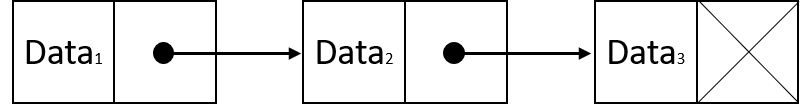
\includegraphics[width=8.00cm, height=1.04cm]{figures/linked_list}
	\end{center}
	\caption{Linked List}
	\label{figure_linked_list} 
\end{figure}

For traversing the list, or lookup, this would take at most a number of operations equal to the length of the list. This is because each element must be looked at in order. Therefore, lookups take O(n) time - a time proportional to the number of items stored in the list.

\subsubsection{Binary Search Trees}
Going back as far as 1960, these are tree data structure where each node has at most 2 children. This is comparable to a linked list, but has two pointers to two different nodes instead of one. The definition of this data structure requires that upon inserting a new node, it should be placed on one side of the tree based on some comparison - for numbers, this can perhaps be comparing size. To search or insert a given node, one must traverse, on average, nodes equal to the logarithm of the number of items stored in the tree. Therefore, lookup and insertion takes O(log n) time.

Binary Search Trees are most efficient when evenly balanced; i.e, the left hand side of a tree has roughly equal nodes to the right hand side. If the tree were to be heavily loaded one side, lookups would generally take longer. Algorithms exist to 'balance' the tree, allowing for faster lookups. However, seeing as though the data structures will be cleared every alloted time period (5 minutes as before), this is less of an issue. This data structure is an attractive choice as it is easy to implement due to its simplicity and is more efficient than a linked list. 
\begin{figure}[h]
	\begin{center}
		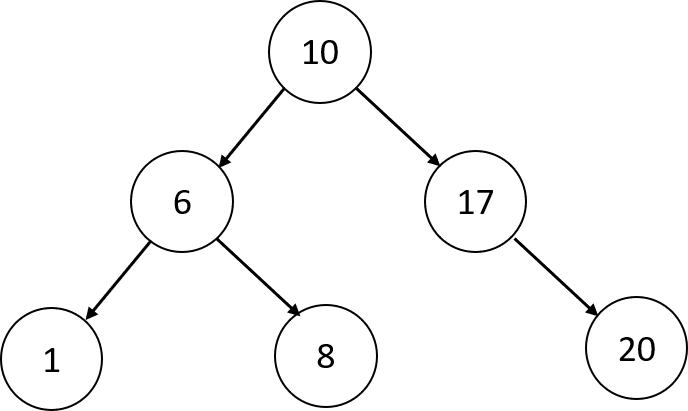
\includegraphics[width=6.68cm, height=4.11cm]{figures/bst}
	\end{center}
	\caption{Binary Search Tree}
	\label{figure_bst} 
\end{figure}

\subsubsection{Hash Table}
A Hash Table is a data structure implementing an associative array, a structure consisting of pairs of exclusive keys and values. To compute the index of a key, a special function called the hash function is used. To lookup a key-value pair, one would compute the hash function of the key and lookup that index. Therefore, in an ideal hash table, the lookup speed would be O(1) as only one operation is needed. 

In the case of source addresses mapping to TTLs, the key would be the source address and the value would be the TTL array. The problem, however, lies in a suitable hash function for the source address. In the simplest case, the hash function would be $f(x) = x$, so the key is the IP address itself. Yet this would mean the hash table would have to be size of the maximum IP address. Being a 32-bit field, the hash table have roughly 4.3 billion entries. Seeing as traversing the table is O(n), this is infeasible.

Having a smaller, more manageable size hash table (1GB perhaps) will result in there being less spaces, or buckets, for keys than there are different possible IP addresses. The hash function will have to map more than one IP address to the same value - when this happens in practice, it is called a collision, and reduces the effectiveness and speed of the hash table. The bigger the hash table, the less likely this is to happen. However, this is limited by memory and the time taken to traverse the table (still being O(n)).

The best hash function to use is one that results in the least number of collisions. Because it is not currently possible to know the distribution of addresses, an effective hash function is very difficult to create.

\subsubsection{Judy Array\cite{judy}}
Invented by Douglas Baskins and named after his sister, a Judy array is another type of associative array made popular by its highly optimised performance and low memory usage. Unlike many associative arrays, Judy arrays do not use hashing. They can efficiently represent sparse data; can scale up to very large numbers, bound only by machine memory; and are not pre-allocated, but grows and shrinks dynamically.   

Due to being designed to maximise usage of the CPU cache, Judy arrays lookups are near O($\log_{256} n$)\cite{judy256}, usually faster than B-Trees and Hash tables. The downside to Judy Arrays are that they are extremely complex, the smallest implementations requiring thousands of lines of code. All current implementations of Judy Arrays available offer no method of being used in Kernel space. 

\subsubsection{Conclusion}
Hash Tables and Judy Arrays are enticing options due to their fast lookup speeds. Although Hash Tables come with slow Traversal speeds, this is much less concerning than lookup speed, as this only has to be done every time segment when the data is sent to userpace and aggregated into a database. Although, having traversal speeds so slow as to traverse many millions of entries, this could be incredibly detrimental.

Development time is also of concern - creating an effective hash function without data is a difficult and possibly fruitless task. Furthermore, implementing a Judy Array in kernel space would be a mammoth undertaking as current implementations only state for use in userspace.

Binary Search trees are quick and easy to implement, whilst still looking very efficient. For this purpose, they are strictly better than linked lists due to their faster lookup speeds. Therefore, for the time being, a binary search tree will be the choice of data structure to hold source IP addresses, protocol and TTL's in kernel space.

%%%%%%%%%%%%%%%%%%%%%%%%%%%%%%%%%%%%%%%%%%%%%%%%%%%%%%%%%%%%%%%%%%%%%%
\subsection{Multiple Writers Problem}

It was mentioned that it is efficient to utilise all processing power by have multiple threads taking work out of a workqueue and processing it concurrently. However, having multiple threads manipulating the same data structure introduces race conditions - behaviour dependent on the sequence or timing of uncontrollable events. For example, if two threads, t1 and t2, are traversing a binary search tree and trying to insert two different nodes, n1 and n2 respectively, perhaps they need to be inserted into the exact same position - say, the left child of n3. The execution order of the threads is undefined, so it could occur that both threads have traversed the tree and decided that the node needs to lie to the left of node n3, but have not yet inserted. When the threads go to insert their node, t1 could make the left child of n3 point to n1, and immediately after, t2 could also make the left child of n3 point to n2, overriding the previous assignment and completely losing n1, making it unreachable.. 

One solution is to initialise a mutual exclusion lock (mutex) that must be acquired before accessing the data structure. Only one thread at any given point can hold the lock, and a thread can only use the tree if it holds the lock. This ensures there is never a point where two or more threads are accessing the same data structure.

Although this eliminates all possible race conditions that might occur, it subsequently enforces a linear flow of execution amongst the threads. This is because the thread's only job is to traverse the tree and insert nodes, so mutex locks would ensure only one thread is executing at any time - completely invalidating any benefits of using threads.

A method is needed to enable multiple writers of data with no race conditions. To ensure this on the same, ever increasing data structure is a very difficult task. Instead, we can simply have multiple data structures. The solution chosen was to have work evenly distributed to multiple trees, so each thread can work on a different tree. This enables concurrency whilst preventing race conditions.

As we cannot guarantee which tree the data is inserted into, having multiple trees introduces the problem of duplicate entries for a source address. Although, implementing a mechanism to avoid this would require another data structure with checks, taking up valuable time. Because the data is only collected and inserted into the database every time interval, we can easily just sort out duplicate entries and aggregate the data at a later stage.

\begin{figure}[h]
	\begin{center}
		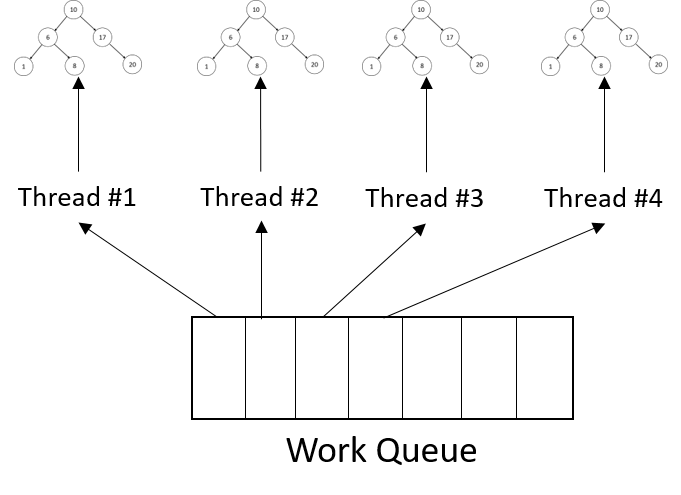
\includegraphics[width=6.81cm, height=4.95cm]{figures/trees}
	\end{center}
	\caption{Multiple threads working on multiple trees concurrently}
	\label{figure_trees} 
\end{figure}

%%%%%%%%%%%%%%%%%%%%%%%%%%%%%%%%%%%%%%%%%%%%%%%%%%%%%%%%%%%%%%%%%%%%%%
\section{Directions for Future Work}
Being a work in progress report, there are still many areas to explore. The next step is to deploy the data collection tool and observe how it handles large data tools. If it is the case that the tool is unable to handle the maximum data stream, then more efforts must be made to decrease the time handling the data.

\subsection{More Efficient Data Structure}
As discussed in section \ref{data_structures}, there are more efficient data structures than the currently used binary search tree. For example, when implemented correctly, hash tables make for a great choice. When enough data is collected, an efficient hashing function could be developed to allow hash tables to operate even faster than binary search trees.

It is also theoretically possible to implement a Judy Array in kernel space. Although difficult, doing so would result in significant performance increase. How much so, and if it even is required, can only be known once the current implementation is observed working.

\subsection{Classifying Correctness}
Once sufficient data is collected, tests must be carried out to calculate the predictability of TTL values for a given IP. For example, as seen before, the conditional entropy of the values could be used. Alternatively, a simple variance can be calculated.

Machine learning classification techniques, namely a naïve Bayes classifier\cite{naive}, will be used to differentiate legitimate sources from illegitimate ones. This is a simple and effective probabilistic classifier based on Bayes Theorem. It assumes independence between events - that is, the outcome of one event does not influence the others. In the case of separate IP requests with several TTL values, these are entirely independent, so this assumption holds.

The cost associated with allowing a fake packet to pass is far less than denying a legitimate user access. It is imperative to reduce the number of false positives, i.e. class a legitimate packet as spoofed and discard it. As long as most spoofed packets are detected, this will decrease the effectiveness of DDoS attacks considerably. Therefore, statistical evaluation metrics, such as K-fold cross validation\cite{kfold}, will be the primary way of testing the accuracy of the classifier. This is a widely used technique to evaluate predictive models by recursively partitioning the data set into a training set to train the model, and a test set to judge its effectiveness. 

\subsection{Tool Implementation}
If all goes perfectly well, an extension to this project is to actually build an implement this work real-time. A tool would sit and look at every packet - similar to the data collection tool - and make a decision on every packet as to whether it's spoofed or not. This would happen simultaneously to logging the packets in the database.

As a lot of time has been spent developing a tool to efficiently log datagrams, this can be used as a platform to simply expand upon to incorporate the classification. Though more development time would have to be spend on making the classification as quick and efficient as possible.

%%%%%%%%%%%%%%%%%%%%%%%%%%%%%%%%%%%%%%%%%%%%%%%%%%%%%%%%%%%%%%%%%%%%%%


\bibliographystyle{asmems4}

\bibliography{scientificPaperBib}

\end{document}
